
% Default to the notebook output style

    


% Inherit from the specified cell style.




    
\documentclass[11pt]{article}

    
    
    \usepackage[T1]{fontenc}
    % Nicer default font (+ math font) than Computer Modern for most use cases
    \usepackage{mathpazo}

    % Basic figure setup, for now with no caption control since it's done
    % automatically by Pandoc (which extracts ![](path) syntax from Markdown).
    \usepackage{graphicx}
    % We will generate all images so they have a width \maxwidth. This means
    % that they will get their normal width if they fit onto the page, but
    % are scaled down if they would overflow the margins.
    \makeatletter
    \def\maxwidth{\ifdim\Gin@nat@width>\linewidth\linewidth
    \else\Gin@nat@width\fi}
    \makeatother
    \let\Oldincludegraphics\includegraphics
    % Set max figure width to be 80% of text width, for now hardcoded.
    \renewcommand{\includegraphics}[1]{\Oldincludegraphics[width=.8\maxwidth]{#1}}
    % Ensure that by default, figures have no caption (until we provide a
    % proper Figure object with a Caption API and a way to capture that
    % in the conversion process - todo).
    \usepackage{caption}
    \DeclareCaptionLabelFormat{nolabel}{}
    \captionsetup{labelformat=nolabel}

    \usepackage{adjustbox} % Used to constrain images to a maximum size 
    \usepackage{xcolor} % Allow colors to be defined
    \usepackage{enumerate} % Needed for markdown enumerations to work
    \usepackage{geometry} % Used to adjust the document margins
    \usepackage{amsmath} % Equations
    \usepackage{amssymb} % Equations
    \usepackage{textcomp} % defines textquotesingle
    % Hack from http://tex.stackexchange.com/a/47451/13684:
    \AtBeginDocument{%
        \def\PYZsq{\textquotesingle}% Upright quotes in Pygmentized code
    }
    \usepackage{upquote} % Upright quotes for verbatim code
    \usepackage{eurosym} % defines \euro
    \usepackage[mathletters]{ucs} % Extended unicode (utf-8) support
    \usepackage[utf8x]{inputenc} % Allow utf-8 characters in the tex document
    \usepackage{fancyvrb} % verbatim replacement that allows latex
    \usepackage{grffile} % extends the file name processing of package graphics 
                         % to support a larger range 
    % The hyperref package gives us a pdf with properly built
    % internal navigation ('pdf bookmarks' for the table of contents,
    % internal cross-reference links, web links for URLs, etc.)
    \usepackage{hyperref}
    \usepackage{longtable} % longtable support required by pandoc >1.10
    \usepackage{booktabs}  % table support for pandoc > 1.12.2
    \usepackage[inline]{enumitem} % IRkernel/repr support (it uses the enumerate* environment)
    \usepackage[normalem]{ulem} % ulem is needed to support strikethroughs (\sout)
                                % normalem makes italics be italics, not underlines
    

    
    
    % Colors for the hyperref package
    \definecolor{urlcolor}{rgb}{0,.145,.698}
    \definecolor{linkcolor}{rgb}{.71,0.21,0.01}
    \definecolor{citecolor}{rgb}{.12,.54,.11}

    % ANSI colors
    \definecolor{ansi-black}{HTML}{3E424D}
    \definecolor{ansi-black-intense}{HTML}{282C36}
    \definecolor{ansi-red}{HTML}{E75C58}
    \definecolor{ansi-red-intense}{HTML}{B22B31}
    \definecolor{ansi-green}{HTML}{00A250}
    \definecolor{ansi-green-intense}{HTML}{007427}
    \definecolor{ansi-yellow}{HTML}{DDB62B}
    \definecolor{ansi-yellow-intense}{HTML}{B27D12}
    \definecolor{ansi-blue}{HTML}{208FFB}
    \definecolor{ansi-blue-intense}{HTML}{0065CA}
    \definecolor{ansi-magenta}{HTML}{D160C4}
    \definecolor{ansi-magenta-intense}{HTML}{A03196}
    \definecolor{ansi-cyan}{HTML}{60C6C8}
    \definecolor{ansi-cyan-intense}{HTML}{258F8F}
    \definecolor{ansi-white}{HTML}{C5C1B4}
    \definecolor{ansi-white-intense}{HTML}{A1A6B2}

    % commands and environments needed by pandoc snippets
    % extracted from the output of `pandoc -s`
    \providecommand{\tightlist}{%
      \setlength{\itemsep}{0pt}\setlength{\parskip}{0pt}}
    \DefineVerbatimEnvironment{Highlighting}{Verbatim}{commandchars=\\\{\}}
    % Add ',fontsize=\small' for more characters per line
    \newenvironment{Shaded}{}{}
    \newcommand{\KeywordTok}[1]{\textcolor[rgb]{0.00,0.44,0.13}{\textbf{{#1}}}}
    \newcommand{\DataTypeTok}[1]{\textcolor[rgb]{0.56,0.13,0.00}{{#1}}}
    \newcommand{\DecValTok}[1]{\textcolor[rgb]{0.25,0.63,0.44}{{#1}}}
    \newcommand{\BaseNTok}[1]{\textcolor[rgb]{0.25,0.63,0.44}{{#1}}}
    \newcommand{\FloatTok}[1]{\textcolor[rgb]{0.25,0.63,0.44}{{#1}}}
    \newcommand{\CharTok}[1]{\textcolor[rgb]{0.25,0.44,0.63}{{#1}}}
    \newcommand{\StringTok}[1]{\textcolor[rgb]{0.25,0.44,0.63}{{#1}}}
    \newcommand{\CommentTok}[1]{\textcolor[rgb]{0.38,0.63,0.69}{\textit{{#1}}}}
    \newcommand{\OtherTok}[1]{\textcolor[rgb]{0.00,0.44,0.13}{{#1}}}
    \newcommand{\AlertTok}[1]{\textcolor[rgb]{1.00,0.00,0.00}{\textbf{{#1}}}}
    \newcommand{\FunctionTok}[1]{\textcolor[rgb]{0.02,0.16,0.49}{{#1}}}
    \newcommand{\RegionMarkerTok}[1]{{#1}}
    \newcommand{\ErrorTok}[1]{\textcolor[rgb]{1.00,0.00,0.00}{\textbf{{#1}}}}
    \newcommand{\NormalTok}[1]{{#1}}
    
    % Additional commands for more recent versions of Pandoc
    \newcommand{\ConstantTok}[1]{\textcolor[rgb]{0.53,0.00,0.00}{{#1}}}
    \newcommand{\SpecialCharTok}[1]{\textcolor[rgb]{0.25,0.44,0.63}{{#1}}}
    \newcommand{\VerbatimStringTok}[1]{\textcolor[rgb]{0.25,0.44,0.63}{{#1}}}
    \newcommand{\SpecialStringTok}[1]{\textcolor[rgb]{0.73,0.40,0.53}{{#1}}}
    \newcommand{\ImportTok}[1]{{#1}}
    \newcommand{\DocumentationTok}[1]{\textcolor[rgb]{0.73,0.13,0.13}{\textit{{#1}}}}
    \newcommand{\AnnotationTok}[1]{\textcolor[rgb]{0.38,0.63,0.69}{\textbf{\textit{{#1}}}}}
    \newcommand{\CommentVarTok}[1]{\textcolor[rgb]{0.38,0.63,0.69}{\textbf{\textit{{#1}}}}}
    \newcommand{\VariableTok}[1]{\textcolor[rgb]{0.10,0.09,0.49}{{#1}}}
    \newcommand{\ControlFlowTok}[1]{\textcolor[rgb]{0.00,0.44,0.13}{\textbf{{#1}}}}
    \newcommand{\OperatorTok}[1]{\textcolor[rgb]{0.40,0.40,0.40}{{#1}}}
    \newcommand{\BuiltInTok}[1]{{#1}}
    \newcommand{\ExtensionTok}[1]{{#1}}
    \newcommand{\PreprocessorTok}[1]{\textcolor[rgb]{0.74,0.48,0.00}{{#1}}}
    \newcommand{\AttributeTok}[1]{\textcolor[rgb]{0.49,0.56,0.16}{{#1}}}
    \newcommand{\InformationTok}[1]{\textcolor[rgb]{0.38,0.63,0.69}{\textbf{\textit{{#1}}}}}
    \newcommand{\WarningTok}[1]{\textcolor[rgb]{0.38,0.63,0.69}{\textbf{\textit{{#1}}}}}
    
    
    % Define a nice break command that doesn't care if a line doesn't already
    % exist.
    \def\br{\hspace*{\fill} \\* }
    % Math Jax compatability definitions
    \def\gt{>}
    \def\lt{<}
    % Document parameters
    \title{program\_list}
    
    
    

    % Pygments definitions
    
\makeatletter
\def\PY@reset{\let\PY@it=\relax \let\PY@bf=\relax%
    \let\PY@ul=\relax \let\PY@tc=\relax%
    \let\PY@bc=\relax \let\PY@ff=\relax}
\def\PY@tok#1{\csname PY@tok@#1\endcsname}
\def\PY@toks#1+{\ifx\relax#1\empty\else%
    \PY@tok{#1}\expandafter\PY@toks\fi}
\def\PY@do#1{\PY@bc{\PY@tc{\PY@ul{%
    \PY@it{\PY@bf{\PY@ff{#1}}}}}}}
\def\PY#1#2{\PY@reset\PY@toks#1+\relax+\PY@do{#2}}

\expandafter\def\csname PY@tok@nb\endcsname{\def\PY@tc##1{\textcolor[rgb]{0.00,0.50,0.00}{##1}}}
\expandafter\def\csname PY@tok@nl\endcsname{\def\PY@tc##1{\textcolor[rgb]{0.63,0.63,0.00}{##1}}}
\expandafter\def\csname PY@tok@s\endcsname{\def\PY@tc##1{\textcolor[rgb]{0.73,0.13,0.13}{##1}}}
\expandafter\def\csname PY@tok@gh\endcsname{\let\PY@bf=\textbf\def\PY@tc##1{\textcolor[rgb]{0.00,0.00,0.50}{##1}}}
\expandafter\def\csname PY@tok@gi\endcsname{\def\PY@tc##1{\textcolor[rgb]{0.00,0.63,0.00}{##1}}}
\expandafter\def\csname PY@tok@w\endcsname{\def\PY@tc##1{\textcolor[rgb]{0.73,0.73,0.73}{##1}}}
\expandafter\def\csname PY@tok@ne\endcsname{\let\PY@bf=\textbf\def\PY@tc##1{\textcolor[rgb]{0.82,0.25,0.23}{##1}}}
\expandafter\def\csname PY@tok@k\endcsname{\let\PY@bf=\textbf\def\PY@tc##1{\textcolor[rgb]{0.00,0.50,0.00}{##1}}}
\expandafter\def\csname PY@tok@sb\endcsname{\def\PY@tc##1{\textcolor[rgb]{0.73,0.13,0.13}{##1}}}
\expandafter\def\csname PY@tok@kp\endcsname{\def\PY@tc##1{\textcolor[rgb]{0.00,0.50,0.00}{##1}}}
\expandafter\def\csname PY@tok@vm\endcsname{\def\PY@tc##1{\textcolor[rgb]{0.10,0.09,0.49}{##1}}}
\expandafter\def\csname PY@tok@vi\endcsname{\def\PY@tc##1{\textcolor[rgb]{0.10,0.09,0.49}{##1}}}
\expandafter\def\csname PY@tok@gp\endcsname{\let\PY@bf=\textbf\def\PY@tc##1{\textcolor[rgb]{0.00,0.00,0.50}{##1}}}
\expandafter\def\csname PY@tok@gu\endcsname{\let\PY@bf=\textbf\def\PY@tc##1{\textcolor[rgb]{0.50,0.00,0.50}{##1}}}
\expandafter\def\csname PY@tok@kc\endcsname{\let\PY@bf=\textbf\def\PY@tc##1{\textcolor[rgb]{0.00,0.50,0.00}{##1}}}
\expandafter\def\csname PY@tok@mi\endcsname{\def\PY@tc##1{\textcolor[rgb]{0.40,0.40,0.40}{##1}}}
\expandafter\def\csname PY@tok@mf\endcsname{\def\PY@tc##1{\textcolor[rgb]{0.40,0.40,0.40}{##1}}}
\expandafter\def\csname PY@tok@sx\endcsname{\def\PY@tc##1{\textcolor[rgb]{0.00,0.50,0.00}{##1}}}
\expandafter\def\csname PY@tok@il\endcsname{\def\PY@tc##1{\textcolor[rgb]{0.40,0.40,0.40}{##1}}}
\expandafter\def\csname PY@tok@ss\endcsname{\def\PY@tc##1{\textcolor[rgb]{0.10,0.09,0.49}{##1}}}
\expandafter\def\csname PY@tok@na\endcsname{\def\PY@tc##1{\textcolor[rgb]{0.49,0.56,0.16}{##1}}}
\expandafter\def\csname PY@tok@ch\endcsname{\let\PY@it=\textit\def\PY@tc##1{\textcolor[rgb]{0.25,0.50,0.50}{##1}}}
\expandafter\def\csname PY@tok@kt\endcsname{\def\PY@tc##1{\textcolor[rgb]{0.69,0.00,0.25}{##1}}}
\expandafter\def\csname PY@tok@sd\endcsname{\let\PY@it=\textit\def\PY@tc##1{\textcolor[rgb]{0.73,0.13,0.13}{##1}}}
\expandafter\def\csname PY@tok@se\endcsname{\let\PY@bf=\textbf\def\PY@tc##1{\textcolor[rgb]{0.73,0.40,0.13}{##1}}}
\expandafter\def\csname PY@tok@ow\endcsname{\let\PY@bf=\textbf\def\PY@tc##1{\textcolor[rgb]{0.67,0.13,1.00}{##1}}}
\expandafter\def\csname PY@tok@gs\endcsname{\let\PY@bf=\textbf}
\expandafter\def\csname PY@tok@cm\endcsname{\let\PY@it=\textit\def\PY@tc##1{\textcolor[rgb]{0.25,0.50,0.50}{##1}}}
\expandafter\def\csname PY@tok@o\endcsname{\def\PY@tc##1{\textcolor[rgb]{0.40,0.40,0.40}{##1}}}
\expandafter\def\csname PY@tok@nn\endcsname{\let\PY@bf=\textbf\def\PY@tc##1{\textcolor[rgb]{0.00,0.00,1.00}{##1}}}
\expandafter\def\csname PY@tok@mh\endcsname{\def\PY@tc##1{\textcolor[rgb]{0.40,0.40,0.40}{##1}}}
\expandafter\def\csname PY@tok@m\endcsname{\def\PY@tc##1{\textcolor[rgb]{0.40,0.40,0.40}{##1}}}
\expandafter\def\csname PY@tok@fm\endcsname{\def\PY@tc##1{\textcolor[rgb]{0.00,0.00,1.00}{##1}}}
\expandafter\def\csname PY@tok@s2\endcsname{\def\PY@tc##1{\textcolor[rgb]{0.73,0.13,0.13}{##1}}}
\expandafter\def\csname PY@tok@nd\endcsname{\def\PY@tc##1{\textcolor[rgb]{0.67,0.13,1.00}{##1}}}
\expandafter\def\csname PY@tok@kd\endcsname{\let\PY@bf=\textbf\def\PY@tc##1{\textcolor[rgb]{0.00,0.50,0.00}{##1}}}
\expandafter\def\csname PY@tok@go\endcsname{\def\PY@tc##1{\textcolor[rgb]{0.53,0.53,0.53}{##1}}}
\expandafter\def\csname PY@tok@ni\endcsname{\let\PY@bf=\textbf\def\PY@tc##1{\textcolor[rgb]{0.60,0.60,0.60}{##1}}}
\expandafter\def\csname PY@tok@sr\endcsname{\def\PY@tc##1{\textcolor[rgb]{0.73,0.40,0.53}{##1}}}
\expandafter\def\csname PY@tok@vg\endcsname{\def\PY@tc##1{\textcolor[rgb]{0.10,0.09,0.49}{##1}}}
\expandafter\def\csname PY@tok@c1\endcsname{\let\PY@it=\textit\def\PY@tc##1{\textcolor[rgb]{0.25,0.50,0.50}{##1}}}
\expandafter\def\csname PY@tok@sh\endcsname{\def\PY@tc##1{\textcolor[rgb]{0.73,0.13,0.13}{##1}}}
\expandafter\def\csname PY@tok@c\endcsname{\let\PY@it=\textit\def\PY@tc##1{\textcolor[rgb]{0.25,0.50,0.50}{##1}}}
\expandafter\def\csname PY@tok@s1\endcsname{\def\PY@tc##1{\textcolor[rgb]{0.73,0.13,0.13}{##1}}}
\expandafter\def\csname PY@tok@kr\endcsname{\let\PY@bf=\textbf\def\PY@tc##1{\textcolor[rgb]{0.00,0.50,0.00}{##1}}}
\expandafter\def\csname PY@tok@mo\endcsname{\def\PY@tc##1{\textcolor[rgb]{0.40,0.40,0.40}{##1}}}
\expandafter\def\csname PY@tok@no\endcsname{\def\PY@tc##1{\textcolor[rgb]{0.53,0.00,0.00}{##1}}}
\expandafter\def\csname PY@tok@sa\endcsname{\def\PY@tc##1{\textcolor[rgb]{0.73,0.13,0.13}{##1}}}
\expandafter\def\csname PY@tok@si\endcsname{\let\PY@bf=\textbf\def\PY@tc##1{\textcolor[rgb]{0.73,0.40,0.53}{##1}}}
\expandafter\def\csname PY@tok@cs\endcsname{\let\PY@it=\textit\def\PY@tc##1{\textcolor[rgb]{0.25,0.50,0.50}{##1}}}
\expandafter\def\csname PY@tok@nc\endcsname{\let\PY@bf=\textbf\def\PY@tc##1{\textcolor[rgb]{0.00,0.00,1.00}{##1}}}
\expandafter\def\csname PY@tok@cpf\endcsname{\let\PY@it=\textit\def\PY@tc##1{\textcolor[rgb]{0.25,0.50,0.50}{##1}}}
\expandafter\def\csname PY@tok@kn\endcsname{\let\PY@bf=\textbf\def\PY@tc##1{\textcolor[rgb]{0.00,0.50,0.00}{##1}}}
\expandafter\def\csname PY@tok@ge\endcsname{\let\PY@it=\textit}
\expandafter\def\csname PY@tok@gr\endcsname{\def\PY@tc##1{\textcolor[rgb]{1.00,0.00,0.00}{##1}}}
\expandafter\def\csname PY@tok@nv\endcsname{\def\PY@tc##1{\textcolor[rgb]{0.10,0.09,0.49}{##1}}}
\expandafter\def\csname PY@tok@cp\endcsname{\def\PY@tc##1{\textcolor[rgb]{0.74,0.48,0.00}{##1}}}
\expandafter\def\csname PY@tok@bp\endcsname{\def\PY@tc##1{\textcolor[rgb]{0.00,0.50,0.00}{##1}}}
\expandafter\def\csname PY@tok@nf\endcsname{\def\PY@tc##1{\textcolor[rgb]{0.00,0.00,1.00}{##1}}}
\expandafter\def\csname PY@tok@vc\endcsname{\def\PY@tc##1{\textcolor[rgb]{0.10,0.09,0.49}{##1}}}
\expandafter\def\csname PY@tok@mb\endcsname{\def\PY@tc##1{\textcolor[rgb]{0.40,0.40,0.40}{##1}}}
\expandafter\def\csname PY@tok@err\endcsname{\def\PY@bc##1{\setlength{\fboxsep}{0pt}\fcolorbox[rgb]{1.00,0.00,0.00}{1,1,1}{\strut ##1}}}
\expandafter\def\csname PY@tok@dl\endcsname{\def\PY@tc##1{\textcolor[rgb]{0.73,0.13,0.13}{##1}}}
\expandafter\def\csname PY@tok@gt\endcsname{\def\PY@tc##1{\textcolor[rgb]{0.00,0.27,0.87}{##1}}}
\expandafter\def\csname PY@tok@sc\endcsname{\def\PY@tc##1{\textcolor[rgb]{0.73,0.13,0.13}{##1}}}
\expandafter\def\csname PY@tok@nt\endcsname{\let\PY@bf=\textbf\def\PY@tc##1{\textcolor[rgb]{0.00,0.50,0.00}{##1}}}
\expandafter\def\csname PY@tok@gd\endcsname{\def\PY@tc##1{\textcolor[rgb]{0.63,0.00,0.00}{##1}}}

\def\PYZbs{\char`\\}
\def\PYZus{\char`\_}
\def\PYZob{\char`\{}
\def\PYZcb{\char`\}}
\def\PYZca{\char`\^}
\def\PYZam{\char`\&}
\def\PYZlt{\char`\<}
\def\PYZgt{\char`\>}
\def\PYZsh{\char`\#}
\def\PYZpc{\char`\%}
\def\PYZdl{\char`\$}
\def\PYZhy{\char`\-}
\def\PYZsq{\char`\'}
\def\PYZdq{\char`\"}
\def\PYZti{\char`\~}
% for compatibility with earlier versions
\def\PYZat{@}
\def\PYZlb{[}
\def\PYZrb{]}
\makeatother


    % Exact colors from NB
    \definecolor{incolor}{rgb}{0.0, 0.0, 0.5}
    \definecolor{outcolor}{rgb}{0.545, 0.0, 0.0}



    
    % Prevent overflowing lines due to hard-to-break entities
    \sloppy 
    % Setup hyperref package
    \hypersetup{
      breaklinks=true,  % so long urls are correctly broken across lines
      colorlinks=true,
      urlcolor=urlcolor,
      linkcolor=linkcolor,
      citecolor=citecolor,
      }
    % Slightly bigger margins than the latex defaults
    
    \geometry{verbose,tmargin=1in,bmargin=1in,lmargin=1in,rmargin=1in}
    
    

    \begin{document}
    
    
    \maketitle
    
    

    
    \section{主要程序清单和相应程序简要说明}\label{ux4e3bux8981ux7a0bux5e8fux6e05ux5355ux548cux76f8ux5e94ux7a0bux5e8fux7b80ux8981ux8bf4ux660e}

毕设的程序采用: - \textbf{Python 3.5} - \textbf{Ubuntu 16.04} -
\textbf{PyCharm 2017.3} - \textbf{Jupyter Notebook}

第一个层次为网络的整体的架构,按树形结构表示如下:

\begin{verbatim}
program
├── README.md
├── setup.py
├── examples
└── udntools
\end{verbatim}

文件类型和文件说明如下表所示:

\begin{longtable}[c]{@{}ccc@{}}
\toprule
文件名 & 文件类型 & 文件说明\tabularnewline
\midrule
\endhead
README.md & - & 存放介绍毕设内容的一个超链接\tabularnewline
setup.py & - & 注册编写的包到Python的环境变量列表里\tabularnewline
udntools & d & 超密集组网的工具包,是程序的主要部分\tabularnewline
examples & d & 用于存放应用工具包得到的理论和仿真图\tabularnewline
\bottomrule
\end{longtable}

整个程序为两级架构: - "udntools"
软件包为用于实现网络分析基本功能的库文件集合 - "examples" 为应用
"udntools" 工具包得到的理论与方针分析结果

\textbf{"udntools"} 层将在\textbf{本章}的剩余部分进行介绍,
\textbf{"examples"} 层将在\textbf{下一章}中介绍。

\subsection{"udntools" 工具包}\label{udntools-ux5de5ux5177ux5305}

"udntools"
工具包用于表达基站、用户、信道和网络的特性,为程序的主要部分,其中的内容的树形结构表示如下:

\begin{verbatim}
udntools
├── bs
├── channel
├── __init__.py
├── region
├── ue
└── utils
\end{verbatim}

\begin{longtable}[c]{@{}ccc@{}}
\toprule
文件名 & 文件类型 & 文件说明\tabularnewline
\midrule
\endhead
bs & d & 表示微基站属性的包\tabularnewline
ue & d & 表示用户的属性的包\tabularnewline
channel & d & 表示信道的特性的包\tabularnewline
region & d & 网络性能仿真的接口\tabularnewline
utils & d & 辅助实现仿真的方法\tabularnewline
\bottomrule
\end{longtable}

下面对上述的 5 个子包分别进行说明:

\subsubsection{"bs" 子包}\label{bs-ux5b50ux5305}

"bs"子包中的内容的树形结构表示如下:

\begin{verbatim}
bs
├── base_bs.py
└── __init__.py
\end{verbatim}

\paragraph{主要的类及类中的对象和方法}\label{ux4e3bux8981ux7684ux7c7bux53caux7c7bux4e2dux7684ux5bf9ux8c61ux548cux65b9ux6cd5}

\begin{itemize}
\tightlist
\item
  BaseBS

  \begin{itemize}
  \tightlist
  \item
    Inherit from class \textbf{Object}
  \end{itemize}
\end{itemize}

\begin{longtable}[c]{@{}ccc@{}}
\toprule
名称 & 类型 & 说明\tabularnewline
\midrule
\endhead
bs\_number\_ & 对象 & 基站的个数\tabularnewline
bs\_power\_ & 对象 & 基站的功率\tabularnewline
bs\_distribution\_ & 对象 & 基站的分布\tabularnewline
bs\_position\_ & 对象 & 基站的位置\tabularnewline
set\_bs\_to\_region & 抽象方法 & 在区域内生成基站\tabularnewline
select\_ue & 抽象方法 & 寻找基站服务的用户集合\tabularnewline
\bottomrule
\end{longtable}

\subsubsection{"ue"子包}\label{ueux5b50ux5305}

"ue"子包用于表征用户的特性,其中的内容的树形结构表示如下:

\begin{verbatim}
ue
├── base_ue.py
└── __init__.py
\end{verbatim}

\paragraph{主要的类及类中的对象和方法}\label{ux4e3bux8981ux7684ux7c7bux53caux7c7bux4e2dux7684ux5bf9ux8c61ux548cux65b9ux6cd5-1}

\begin{itemize}
\tightlist
\item
  BaseUE

  \begin{itemize}
  \tightlist
  \item
    Inherit from class \textbf{Object}
  \end{itemize}
\end{itemize}

\begin{longtable}[c]{@{}ccc@{}}
\toprule
名称 & 类型 & 说明\tabularnewline
\midrule
\endhead
ue\_number\_ & 对象 & 用户的个数\tabularnewline
ue\_distribution\_ & 对象 & 用户的分布\tabularnewline
bs\_position\_ & 对象 & 用户的位置\tabularnewline
set\_ue\_to\_region & 抽象方法 & 在区域内生成用户\tabularnewline
\bottomrule
\end{longtable}

\subsubsection{"Channel" 子包}\label{channel-ux5b50ux5305}

"channel" 子包中的内容的树形结构表示如下:

\begin{verbatim}
channel
├── __init__.py
├── large_fade_channel.py
└── small_fade_channel.py
\end{verbatim}

\paragraph{主要的类及类中的对象和方法}\label{ux4e3bux8981ux7684ux7c7bux53caux7c7bux4e2dux7684ux5bf9ux8c61ux548cux65b9ux6cd5-2}

\begin{itemize}
\tightlist
\item
  LargeFadeChannel

  \begin{itemize}
  \tightlist
  \item
    Inherit from class \textbf{Object}
  \end{itemize}
\end{itemize}

\begin{longtable}[c]{@{}ccc@{}}
\toprule
名称 & 类型 & 说明\tabularnewline
\midrule
\endhead
path\_loss\_factor\_ & 对象 & 大尺度衰落系数\tabularnewline
large\_fade\_factor\_matrix & 方法 &
发射信号经过大尺度衰落后的功率\tabularnewline
\bottomrule
\end{longtable}

\begin{itemize}
\tightlist
\item
  SmallFadeChannel

  \begin{itemize}
  \tightlist
  \item
    Inherit from class \textbf{Object}
  \end{itemize}
\end{itemize}

\begin{longtable}[c]{@{}ccc@{}}
\toprule
名称 & 类型 & 说明\tabularnewline
\midrule
\endhead
small\_fade\_ & 对象 & 小尺度衰落的类型\tabularnewline
h\_matrix\_ & 对象 & 信道系数\tabularnewline
generate\_h\_matrix & 方法 & 生成小尺度衰落系数矩阵\tabularnewline
\bottomrule
\end{longtable}

\subsubsection{"Region" 子包}\label{region-ux5b50ux5305}

"region" 子包中的内容的树形结构表示如下:

\begin{verbatim}
region
├── base_region.py
├── comp_service_region.py
├── __init__.py
└── service_region.py
\end{verbatim}

\paragraph{主要的类及类中的对象和方法}\label{ux4e3bux8981ux7684ux7c7bux53caux7c7bux4e2dux7684ux5bf9ux8c61ux548cux65b9ux6cd5-3}

\begin{itemize}
\tightlist
\item
  BaseRegion

  \begin{itemize}
  \tightlist
  \item
    Inherit from class \textbf{Object}
  \end{itemize}
\end{itemize}

\begin{longtable}[c]{@{}ccc@{}}
\toprule
名称 & 类型 & 说明\tabularnewline
\midrule
\endhead
x\_min & 对象 & 区域的左边界\tabularnewline
x\_max & 对象 & 区域的右边界\tabularnewline
y\_min & 对象 & 区域的下边界\tabularnewline
y\_max & 对象 & 区域的上边界\tabularnewline
ground\_position\_ & 对象 & 用于存放生成的格点坐标\tabularnewline
get\_ground & 方法 & 得到格点坐标的矩阵\tabularnewline
\bottomrule
\end{longtable}

\begin{itemize}
\tightlist
\item
  ServiceRegion

  \begin{itemize}
  \tightlist
  \item
    Inherit from class \textbf{BaseRegion, BaseBS, BaseUE}
  \end{itemize}
\end{itemize}

\begin{longtable}[c]{@{}ccc@{}}
\toprule
名称 & 类型 & 说明\tabularnewline
\midrule
\endhead
bs\_ue\_dict\_ & 对象 & 存放基站对应其所服务的用户的字典\tabularnewline
kill\_ue & 方法 & 删除区域内的用户\tabularnewline
set\_bs\_to\_region & 方法 & 区域内基站部署\tabularnewline
set\_ue\_to\_region & 方法 & 区域内基站部署\tabularnewline
set\_ue\_sigma & 方法 & 设定用户的分散程度\tabularnewline
set\_ue\_distribution & 方法 & 设定用户的分布\tabularnewline
select\_ue & 方法 & 得到bs\_ue\_dict\_\tabularnewline
\bottomrule
\end{longtable}

\begin{itemize}
\tightlist
\item
  CompServiceRegion

  \begin{itemize}
  \tightlist
  \item
    Inherit from class \textbf{ServiceRegion, LargeFadeChannel,
    SmallFadeChannel}
  \end{itemize}
\end{itemize}

\begin{longtable}[c]{@{}ccc@{}}
\toprule
名称 & 类型 & 说明\tabularnewline
\midrule
\endhead
cluster\_set\_ & 对象 & 基站分簇得到的集合\tabularnewline
cluster\_bs\_position\_ & 对象 & 簇内基站的坐标\tabularnewline
cluster\_ue\_set\_ & 对象 & 根据基站分簇结果对用户分簇\tabularnewline
cluster\_ue\_position\_ & 对象 & 簇内用户的坐标\tabularnewline
self.sir\_array & 对象 & 每个用户的信干比性能\tabularnewline
cluster\_by\_kmeans & 方法 & 基于 Kmeans 的基站分簇算法\tabularnewline
cluster\_by\_dfs & 方法 & 基于深度优先搜索的基站分簇算法\tabularnewline
get\_cluster\_ue\_position & 方法 & 得到 cluster\_ue\_set\_ 和
cluster\_ue\_position\_\tabularnewline
zfbf\_equal\_allocation & 方法 & 基于 ZFBF
的多用户联合传输算法\tabularnewline
sir\_array\_sim & 方法 & 得到用户的信干比的性能\tabularnewline
\bottomrule
\end{longtable}

\subsubsection{"utils" 子包}\label{utils-ux5b50ux5305}

"utils" 子包中的内容的树形结构表示如下:

\begin{verbatim}
utils
├── ase_theory.py
├── cdf.py
├── dfs_dict_by_distance.py
├── dim2_distance.py
├── __init__.py
└── pc_theory.py
\end{verbatim}

\begin{longtable}[c]{@{}ccc@{}}
\toprule
文件名 & 文件类型 & 说明\tabularnewline
\midrule
\endhead
ase\_theory.py & - & 用于得到单位面积谱效率的理论值\tabularnewline
cdf.py & - & 用于画概率累计分布函数图\tabularnewline
dfs\_dict\_by\_distance.py & - & 实现深度优先搜索算法\tabularnewline
dim2\_distance.py & - & 计算基站和用户之间的欧式距离\tabularnewline
pc\_theory.py & - & 用于得到区域覆盖率的理论值\tabularnewline
\bottomrule
\end{longtable}

    \section{主要程序的流程图或实现框图}\label{ux4e3bux8981ux7a0bux5e8fux7684ux6d41ux7a0bux56feux6216ux5b9eux73b0ux6846ux56fe}

本章介绍主要程序的流程框图或实现框图,即软件的 \textbf{"examples"}
层的部分, \textbf{examples} 层的主要的模块为:

\begin{verbatim}
examples
├── ase_sim
├── capacity_map
├── clustering_precoding
├── dfs_clustering
├── kmeans_clustering
└── pc_sim
\end{verbatim}

其主要的模块如下表所示:

\begin{longtable}[c]{@{}cc@{}}
\toprule
模块名 & 说明\tabularnewline
\midrule
\endhead
ase\_sim & 单位面积频谱效率的理论仿真\tabularnewline
capacity\_map &
用于得到基站的拓扑结构和网络的遍历容量热力分布图\tabularnewline
clustering\_precoding &
密集热点区域无线网络优化后的覆盖率性能分析\tabularnewline
dfs\_clustering &
基于深度优先搜索的基站分簇算法的算法验证与分析\tabularnewline
kmeans\_clustering & 基于 k -
均值的基站分簇算法的算法验证与分析\tabularnewline
pc\_sim & 用于对密集热点区域无线网络的覆盖率的性能的分析\tabularnewline
\bottomrule
\end{longtable}

下面按以论文为线索依次介绍上述的子模块:

    \subsection{对基站的网络拓扑结构的仿真:}\label{ux5bf9ux57faux7ad9ux7684ux7f51ux7edcux62d3ux6251ux7ed3ux6784ux7684ux4effux771f}

\begin{itemize}
\tightlist
\item
  所属子模块:

  \begin{itemize}
  \tightlist
  \item
    examples/capacity\_map
  \end{itemize}
\item
  对应论文中的 \textbf{图 3-3}
\end{itemize}

仿真的步骤为:

\begin{itemize}
\tightlist
\item
  \textbf{Step 0:} 设置网络的服务区域的边界,设置基站的数量
\item
  \textbf{Step 1:} 生成服从泊松点过程的坐标
\item
  \textbf{Step 2:}
  根据生成的坐标画出基站的网络拓扑图,并画出反应每个微基站服务范围的
  Voronoi 图
\end{itemize}

得到的仿真结果图如下图所示:

\begin{figure}[htbp]
\centering
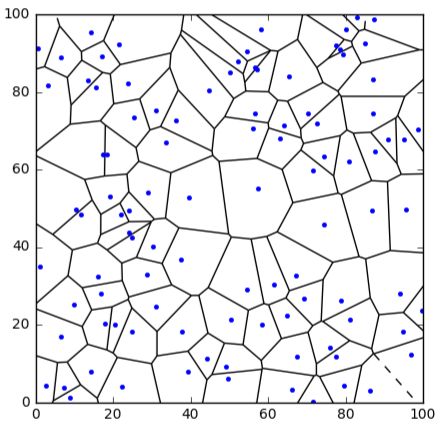
\includegraphics{./bs_station.png}
\caption{基站网络的拓扑结构仿真}
\end{figure}

    \subsection{对网络中各个位置的遍历容量的热力分布图的仿真图:}\label{ux5bf9ux7f51ux7edcux4e2dux5404ux4e2aux4f4dux7f6eux7684ux904dux5386ux5bb9ux91cfux7684ux70edux529bux5206ux5e03ux56feux7684ux4effux771fux56fe}

\begin{itemize}
\tightlist
\item
  所属子模块:

  \begin{itemize}
  \tightlist
  \item
    examples/capacity\_map
  \end{itemize}
\item
  对应论文中的 \textbf{图 3-4}
\end{itemize}

仿真的步骤为: - \textbf{Step 0:}
设置基站拓扑结构,大尺度衰落系数分别设置为2.0和4.0 - \textbf{Step 1:}
对 ground\_position\_
数据结构中的所有坐标求遍历容量,信道是平稳的可以用时间遍历的方法求均值 -
\textbf{Step 2:} 画出基站的热力分布图

得到的仿真结果图如下图所示:

\begin{figure}[htbp]
\centering
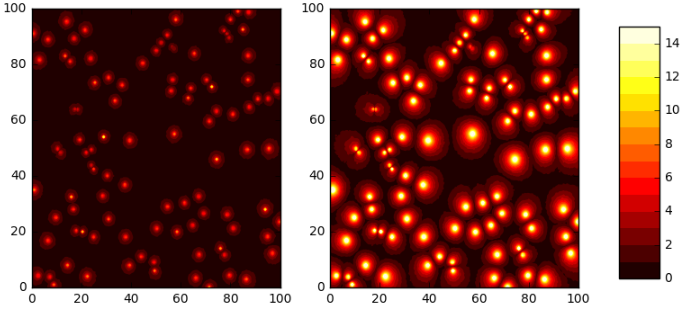
\includegraphics{capacity_hotmap.png}
\caption{capacity\_hotmap}
\end{figure}

    \subsection{对网络的覆盖率的性能的理论分析和仿真:}\label{ux5bf9ux7f51ux7edcux7684ux8986ux76d6ux7387ux7684ux6027ux80fdux7684ux7406ux8bbaux5206ux6790ux548cux4effux771f}

\begin{itemize}
\tightlist
\item
  所属子模块:

  \begin{itemize}
  \tightlist
  \item
    examples/pc\_sim
  \end{itemize}
\item
  对应论文中的 \textbf{图 3-5, 图 3-6, 图 3-7}
\end{itemize}

根据论文中的分析可以得到,在密集热点区域无线网络的场景中,网络的覆盖率上界的表达式,该表达式也为覆盖率的近似式,如下式所示:

\[\tag{1}
P_c(T,\lambda,\alpha,\sigma) =  \frac{1}{1+\rho(T,\alpha)} + \frac{\rho(T, \alpha)}{1+\rho(T,\alpha)} \cdot \frac{1}{2\pi\sigma^2\lambda(1+\rho(T,\alpha))+1}
\]

其中:

\[\tag{2}
\rho(T,\alpha)=T^{2/\alpha}\int_{T^{-2/\alpha}}^{\infty} \frac{1}{1+u^{\alpha/2}}\ \mathrm{d}u
\]

\(P_c\)为覆盖率,\(T\) 为信干比门限,\(\lambda\)
为微基站的密度,\(\alpha\) 为信道的衰落系数,\(\sigma\)
为用户的分散程度。

给出上述表达式的数值解,并和经过蒙特卡洛仿真的到的结果进行对比。

仿真的步骤为: - \textbf{Step 0:} 采用控制变量法,讨论信道衰落系数(
\textbf{图 3-5} ),微基站的密度( \textbf{图 3-6} ),用户分散程度(
\textbf{图 3-7}
)对覆盖率的影响,基站的网络拓扑为泊松点过程,用户的分布为二维高斯分布。
- \textbf{Step 1:} 根据给定的参数对覆盖率性能进行仿真 - \textbf{Step
2:} 根据给定的参数求覆盖率的数值解 - \textbf{Step 3:} 画出曲线对比分析

覆盖率关于信道衰落系数的曲线图如下:

\begin{figure}[htbp]
\centering
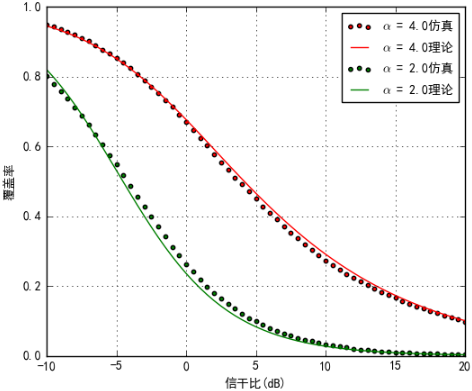
\includegraphics{pc_alpha.png}
\caption{pc\_alpha.png}
\end{figure}

覆盖率关于微基站密度的曲线图如下:

\begin{figure}[htbp]
\centering
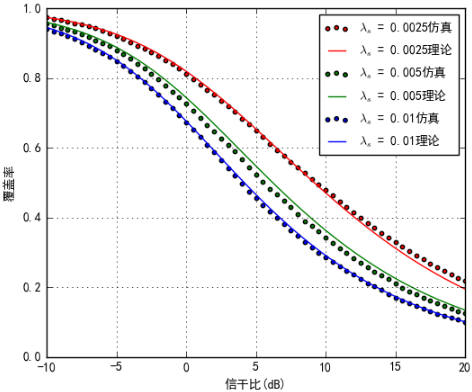
\includegraphics{pc_lambda_s.png}
\caption{pc\_lambda\_s.png}
\end{figure}

覆盖率关于用户分散程度的曲线图如下:

\begin{figure}[htbp]
\centering
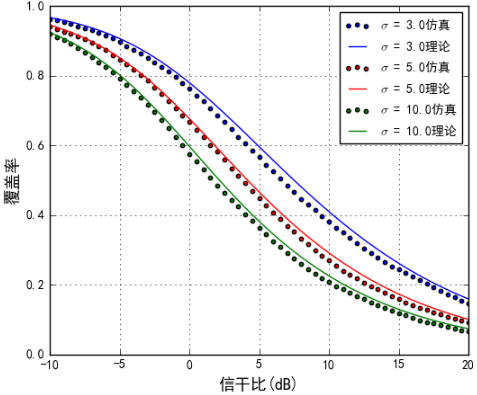
\includegraphics{pc_sigma.png}
\caption{pc\_sigma.png}
\end{figure}

    \subsection{对网络的单位面积谱效率的性能的理论分析:}\label{ux5bf9ux7f51ux7edcux7684ux5355ux4f4dux9762ux79efux8c31ux6548ux7387ux7684ux6027ux80fdux7684ux7406ux8bbaux5206ux6790}

\begin{itemize}
\tightlist
\item
  所属子模块:

  \begin{itemize}
  \tightlist
  \item
    examples/ase\_sim
  \end{itemize}
\item
  对应论文中的 \textbf{图 3-8}
\end{itemize}

根据论文中的分析可以得到区域内单位面积谱效率的表达式如下式所示:

\[\tag{3}
\eta_{ASE} =
\lambda_s\int_{t>0}\frac{1}{1+\rho(2^t-1,\alpha)} + \frac{\rho(2^t-1, \alpha)}{1+\rho(2^t-1,\alpha)} \cdot \frac{1}{2\pi\sigma^2\lambda(1+\rho(2^t-1,\alpha))+1}\ \mathrm{d}t
\]

对其进行数值分析可得到单位面积频谱效率与密度的关系如下图所示:

\begin{figure}[htbp]
\centering
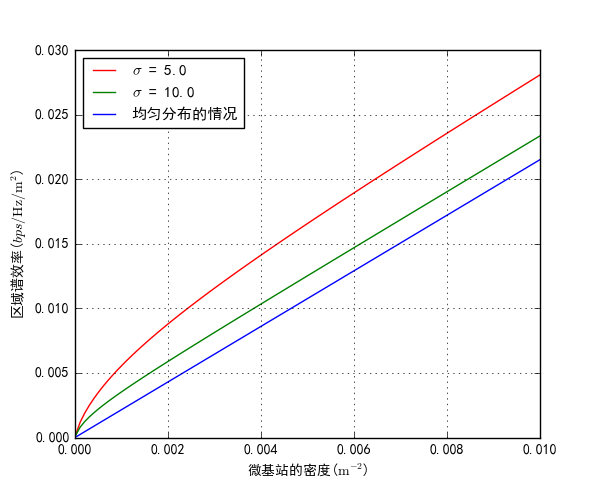
\includegraphics{ase_sigma_lambda.png}
\caption{ase\_sigma\_lambda.png}
\end{figure}

    \subsection{对微基站分簇的仿真示意图:}\label{ux5bf9ux5faeux57faux7ad9ux5206ux7c07ux7684ux4effux771fux793aux610fux56fe}

\subsubsection{基于深度优先搜索的基站分簇算法结果仿真图:}\label{ux57faux4e8eux6df1ux5ea6ux4f18ux5148ux641cux7d22ux7684ux57faux7ad9ux5206ux7c07ux7b97ux6cd5ux7ed3ux679cux4effux771fux56fe}

\begin{itemize}
\tightlist
\item
  所属子模块:

  \begin{itemize}
  \tightlist
  \item
    examples/dfs\_clustering
  \end{itemize}
\item
  对应论文中的 \textbf{图 4-3}
\end{itemize}

仿真的步骤为:

\begin{itemize}
\tightlist
\item
  \textbf{Step 0:} 输入基站拓扑结构,输入距离门限
\item
  \textbf{Step 1:} 使用深度优先搜索算法对基站进行分簇
\item
  \textbf{Step 2:} 画出分簇的仿真结果图
\end{itemize}

得到的结果图如下图所示:

\begin{figure}[htbp]
\centering
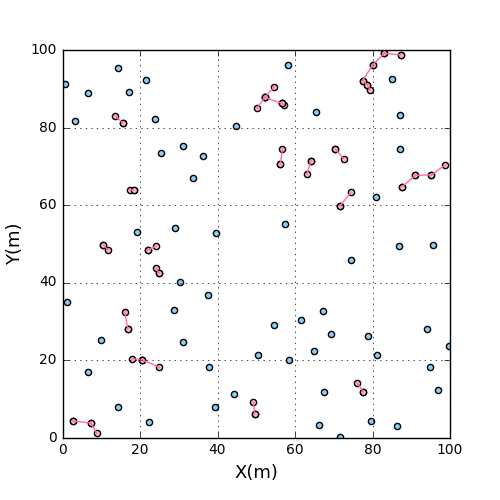
\includegraphics{dfs_network_show.png}
\caption{dfs\_network\_show.png}
\end{figure}

    \subsubsection{基于 k -
均值的基站分簇算法结果仿真图:}\label{ux57faux4e8e-k---ux5747ux503cux7684ux57faux7ad9ux5206ux7c07ux7b97ux6cd5ux7ed3ux679cux4effux771fux56fe}

\begin{itemize}
\tightlist
\item
  所属子模块:

  \begin{itemize}
  \tightlist
  \item
    examples/dfs\_clustering
  \end{itemize}
\item
  对应论文中的 \textbf{图 4-4}
\end{itemize}

仿真的步骤为:

\begin{itemize}
\tightlist
\item
  \textbf{Step 0:} 输入基站拓扑结构,均值个数
\item
  \textbf{Step 1:} 使用 k 均值算法对基站进行分簇
\item
  \textbf{Step 2:} 画出分簇的仿真结果图
\end{itemize}

得到的结果图如下图所示:

\begin{figure}[htbp]
\centering
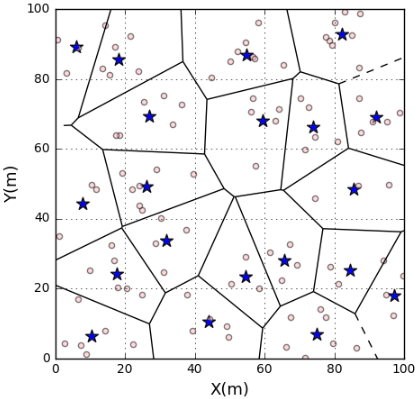
\includegraphics{kmeans_network_show.png}
\caption{kmeans\_network\_show.png}
\end{figure}

    \subsection{对区域内网络性能优化的仿真曲线图:}\label{ux5bf9ux533aux57dfux5185ux7f51ux7edcux6027ux80fdux4f18ux5316ux7684ux4effux771fux66f2ux7ebfux56fe}

\begin{itemize}
\tightlist
\item
  所属子模块:

  \begin{itemize}
  \tightlist
  \item
    examples/clustering\_precoding
  \end{itemize}
\item
  对应论文中的 \textbf{图 4-5, 图 4-6}
\end{itemize}

仿真步骤为:

\begin{itemize}
\tightlist
\item
  \textbf{Step 0:} 输入基站拓扑结构,输入距离门限
\item
  \textbf{Step 1:} 对基站使用深度优先搜索算法( \textbf{图 4-5} ),k -
  均值算法(\textbf{图 4-6})进行分簇
\item
  \textbf{Step 2:} 采用 ZFBF 技术对网络的性能进行优化
\item
  \textbf{Step 3:} 得到优化后的结果
\end{itemize}

使用深度优先搜索算法对基站分簇,再进行性能优化的结果为:

\begin{figure}[htbp]
\centering
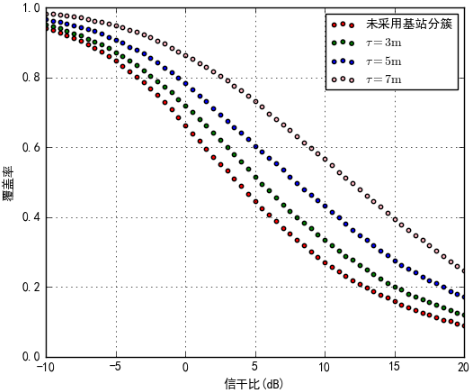
\includegraphics{pc_dfs_zfbf_show.png}
\caption{pc\_dfs\_zfbf\_show.png}
\end{figure}

使用 k 均值算法对基站分簇,再进行性能优化得到的结果为:

\begin{figure}[htbp]
\centering
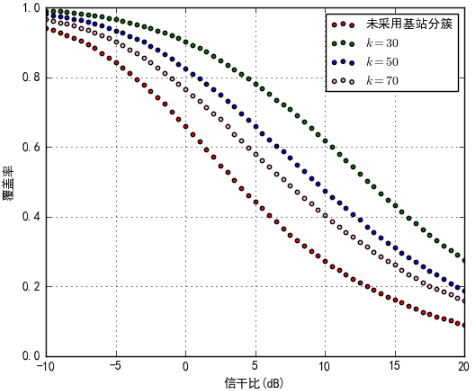
\includegraphics{pc_kmeans_zfbf_show.png}
\caption{pc\_kmeans\_zfbf\_show.png}
\end{figure}

.


    % Add a bibliography block to the postdoc
    
    
    
    \end{document}
